\section{Implementação}

Toda a parte de processamento de imagem se encontra no código fonte \texttt{lib.py}. Cada subseção mostra no trecho de código qual função nesse arquivo se encontra a implementação da operação. Os trechos apresentados refletem o código no arquivo, mas sem detalhes como cópias de \textit{buffer} e tipagem estática.

Quando possível, a função equivalente do OpenCV também será apresentada, já que as acelerações de GPU podem ser facilmente acessadas usando \pyline{cv2.cuda} em vez de apenas \pyline{cv2} \autocite{ref:cvcuda}. Todas as operações também podem ser feitas por uma \textit{lookup table}, com a função \pyline{cv2.LUT} \autocite{ref:LUT} ou a classe \pyline{cv2.cuda.LookUpTable} \autocite{ref:cudaLUT}. Entretanto, as funções deste trabalho foram implementadas apenas com Numpy, visando a familiarização com técnicas de vetorização.

Assuma que as bibliotecas são importadas como:

\begin{minted}{python}
    import numpy as np
    import cv2
\end{minted}

\subsection{Conversão para Monocromático}

A transformação para escala de cinza é feita através da média dos três canais de cores, truncada para inteiro. A matriz resultante é então repetida novamente para os três canais, para que a operação possa ser repetida sem erros de execução do programa.

\begin{listing}[h]
    \caption{Comando \texttt{monocromatico}}

    \begin{minted}{python}
        def grayscale(imagem):
            gray = np.mean(imagem, axis=2).astype(np.uint8)
            return np.stack([gray, gray, gray], axis=2)
    \end{minted}
\end{listing}

\begin{figure}
    \centering
    \begin{subfigure}{0.45\textwidth}
        \centering
        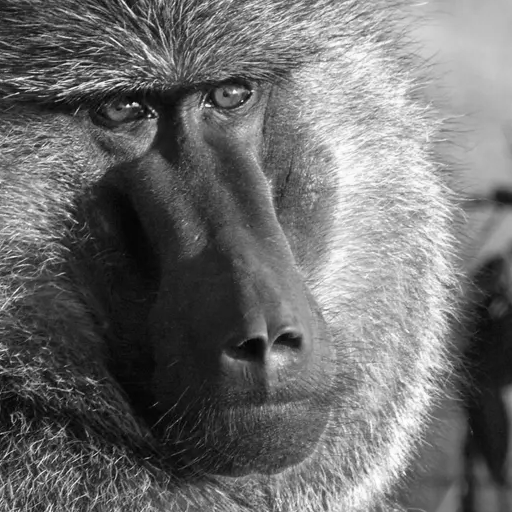
\includegraphics[width=6cm]{resultados/colormono.png}
        \caption{\texttt{imagens/color.png}}
    \end{subfigure}%
    \begin{subfigure}{0.45\textwidth}
        \centering
        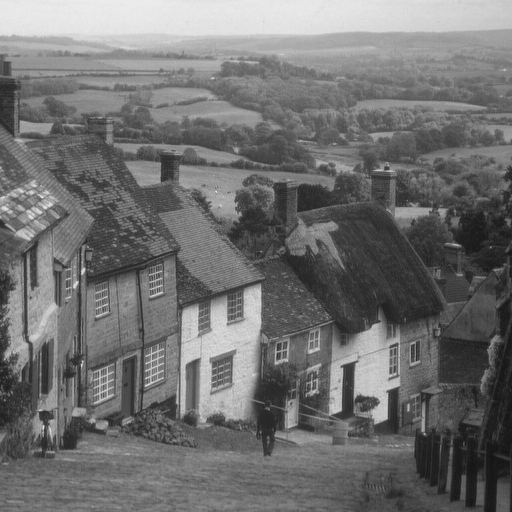
\includegraphics[width=6cm]{resultados/citymono.png}
        \caption{\texttt{imagens/city.png}}
    \end{subfigure}

    \caption{Mudaça para escala de cinza.}
\end{figure}

Em vez de \pyline{np.mean(imagem, ...)}, a conversão poderia ser implementado também com \pyline{cv2.cvtColor(image, cv2.COLOR_BGR2GRAY)} \autocite{ref:cvtcolor}.

\subsection{Negativo da Imagem}

Para essa conversão basta fazer ~\pyline{255 - intensidade}~ para cada píxel. Como 255 também é o maior valor de um \textit{byte}, basta também inverter todos os bits da imagem.

\begin{figure}[H]
    \centering
    \begin{subfigure}{0.45\textwidth}
        \centering
        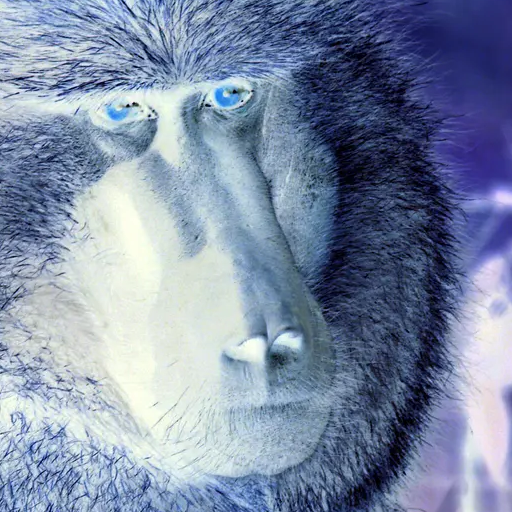
\includegraphics[width=6cm]{resultados/colorneg.png}
        \caption{\texttt{imagens/color.png}}
    \end{subfigure}%
    \begin{subfigure}{0.45\textwidth}
        \centering
        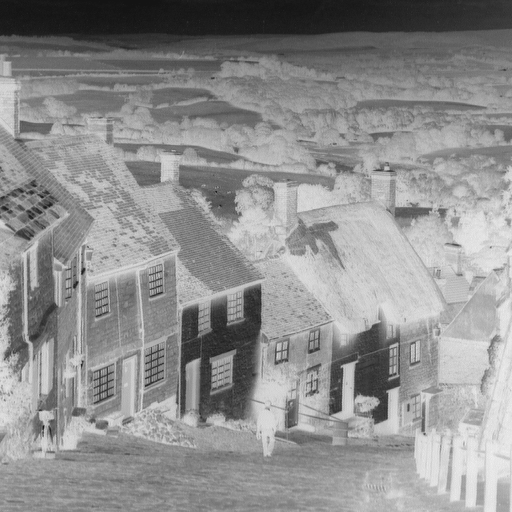
\includegraphics[width=6cm]{resultados/cityneg.png}
        \caption{\texttt{imagens/city.png}}
    \end{subfigure}

    \caption{Imagem com intensidade invertida.}
\end{figure}

\begin{listing}[H]
    \caption{Comando \texttt{negativo}}

    \begin{minted}{python}
        def negativo(imagem):
            return ~imagem
    \end{minted}
\end{listing}

Em vez de usar o \textit{not} do Numpy, existe também a função \pyline{cv2.bitwise_not(imagem)} \autocite{ref:bitwise_not}.

\subsection{Espelhamento Vertical}

\begin{listing}[h]
    \caption{Comando \texttt{esp.vertical}}

    \begin{minted}{python}
        def espelhamento_vertical(imagem):
            return imagem[::-1]
    \end{minted}
\end{listing}

\begin{figure}[h]
    \centering
    \begin{subfigure}{0.45\textwidth}
        \centering
        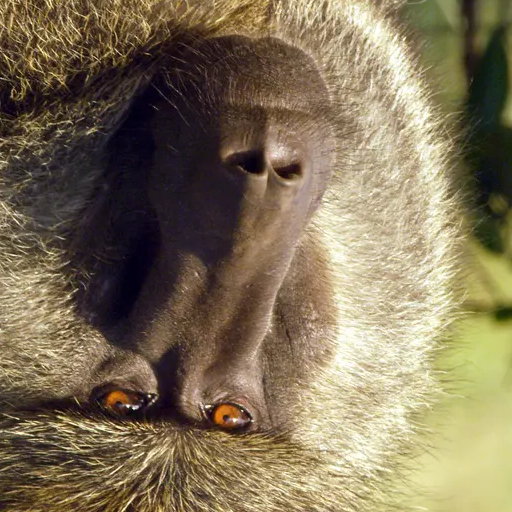
\includegraphics[width=6cm]{resultados/colorflip.png}
        \caption{\texttt{imagens/color.png}}
    \end{subfigure}%
    \begin{subfigure}{0.45\textwidth}
        \centering
        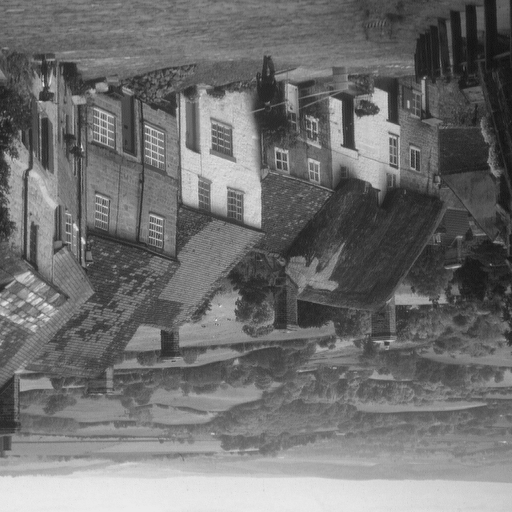
\includegraphics[width=6cm]{resultados/cityflip.png}
        \caption{\texttt{imagens/city.png}}
    \end{subfigure}

    \caption{Espelhamento vertical.}
\end{figure}

Pode ser implementado também com \pyline{cv2.flip(imagem, 0)} \autocite{ref:flip}.

\subsection{Conversão de Intervalo}

Converte o intervalo de intensidade da imagem de [0, 255] para [100, 200] linearmente.

\begin{listing}[h]
    \caption{Comando \texttt{conv.intervalo}}

    \begin{minted}{python}
        def converter_intervalo(imagem):
            zmin, zmax = np.min(imagem), np.max(imagem)
            img = 100 * (image / 255) + 100
            return img.astype(np.uint8)
    \end{minted}
\end{listing}

\begin{figure}[!htb]
    \centering
    \begin{subfigure}{0.45\textwidth}
        \centering
        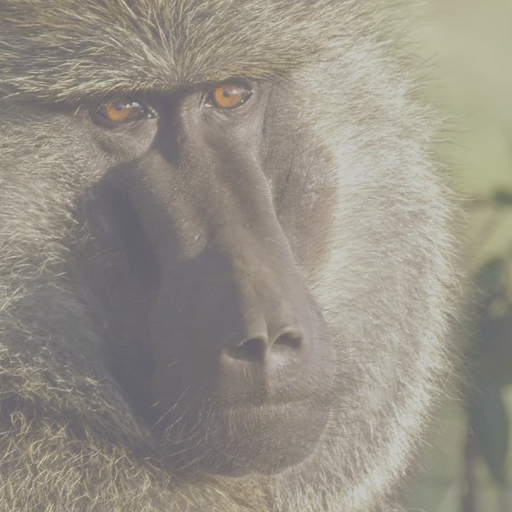
\includegraphics[width=6cm]{resultados/colorconv.png}
        \caption{\texttt{imagens/color.png}}
    \end{subfigure}%
    \begin{subfigure}{0.45\textwidth}
        \centering
        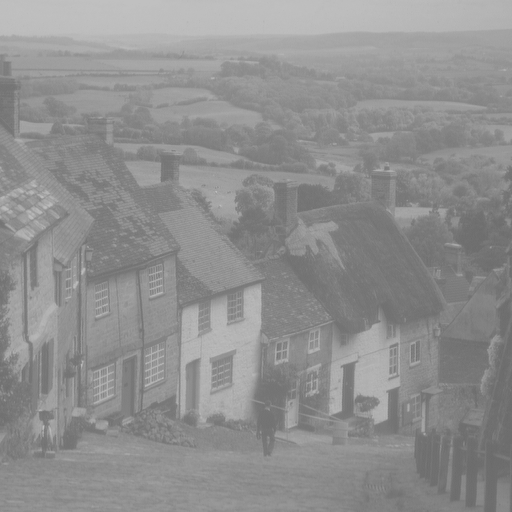
\includegraphics[width=6cm]{resultados/cityconv.png}
        \caption{\texttt{imagens/city.png}}
    \end{subfigure}

    \caption{Intervalo de intensidade convertido.}
\end{figure}

\subsection{Inversão das Linhas Pares}

Inverte todas as linhas pares horizontalmente.

\begin{figure}[h]
    \centering
    \begin{subfigure}{0.45\textwidth}
        \centering
        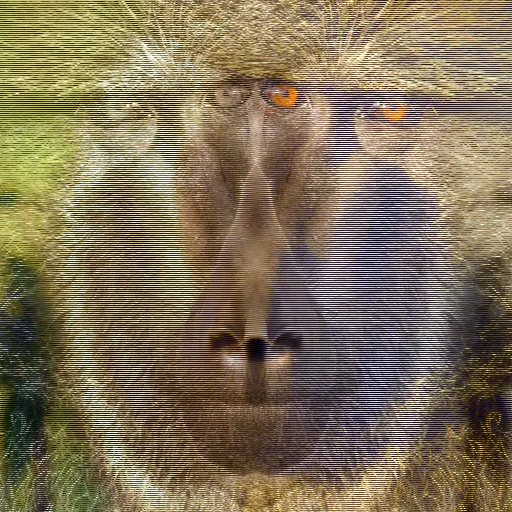
\includegraphics[width=6cm]{resultados/colorinvp.png}
        \caption{\texttt{imagens/color.png}}
    \end{subfigure}%
    \begin{subfigure}{0.45\textwidth}
        \centering
        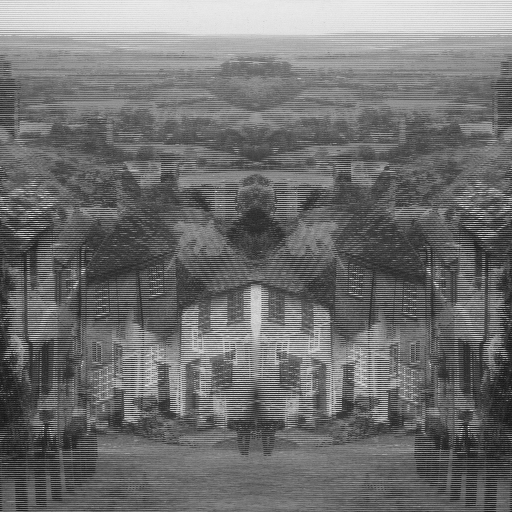
\includegraphics[width=6cm]{resultados/cityinvp.png}
        \caption{\texttt{imagens/city.png}}
    \end{subfigure}

    \caption{Linhas pares invertidas.}
\end{figure}

\begin{listing}[H]

    \begin{minted}{python}
        def inverte_linhas_pares(imagem):
            magem[::2] = image[::2,::-1]
            return imagem
    \end{minted}

    \caption{Comando \texttt{inverte.pares}}
\end{listing}

\subsection{Reflexão das Linhas Superiores}

\begin{listing}[H]
    \begin{minted}{python}
        def reflexao_linhas(imagem):
            mid = len(image) // 2
            imagem[-mid:] = imagem[:mid][::-1]
            return imagem
    \end{minted}

    \caption{Comando \texttt{reflexao}}
\end{listing}

\begin{figure}[H]
    \centering
    \begin{subfigure}{0.45\textwidth}
        \centering
        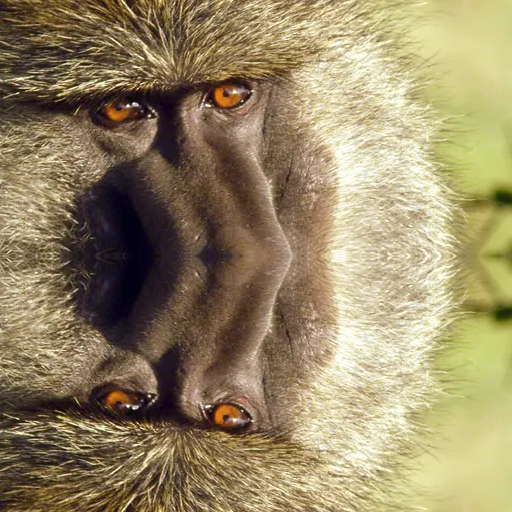
\includegraphics[width=6cm]{resultados/colorrefl.png}
        \caption{\texttt{imagens/color.png}}
    \end{subfigure}%
    \begin{subfigure}{0.45\textwidth}
        \centering
        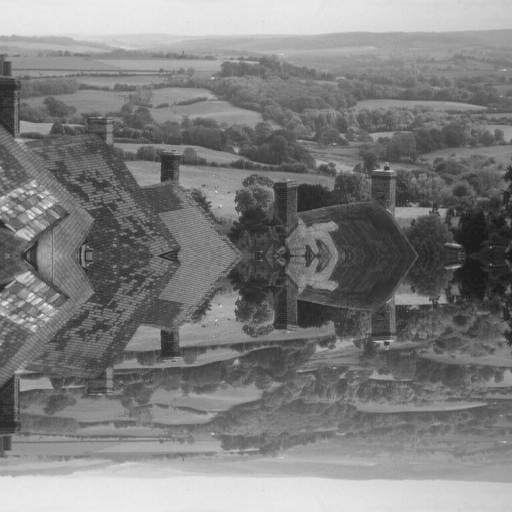
\includegraphics[width=6cm]{resultados/cityrefl.png}
        \caption{\texttt{imagens/city.png}}
    \end{subfigure}

    \caption{Linhas superiores refletidas.}
\end{figure}

\subsection{Ajuste de Brilho}

Ajuste de brilho por correção gama. A implementação é feita convertendo a imagem para uma matriz $A$ com valores em [0, 1]. Com isso, é feita a transformação $B = A^{\frac{1}{\gamma}}$,
sendo $B$ convertida para uma imagem com valores em [0, 255] novamente.

O fator $\gamma$ é passado como argumento para o comando \text{aj.brilho}. Por exemplo, a \cref{fig:ajbrilho} foi feita com o sequinte comando:

\begin{minted}{bash}
    $ python main.py imagens/color.png -o out.png aj.brilho 2.5
\end{minted}

\begin{figure}[H]
    \centering
    \begin{subfigure}{0.45\textwidth}
        \centering
        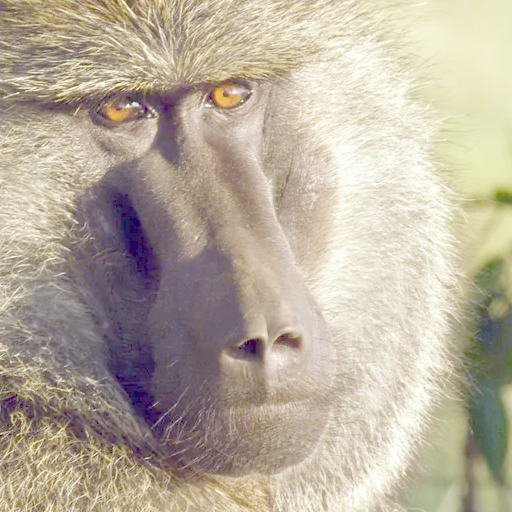
\includegraphics[width=6cm]{resultados/colorgama.png}
        \caption{\texttt{imagens/color.png}}
        \label{fig:ajbrilho}
    \end{subfigure}%
    \begin{subfigure}{0.45\textwidth}
        \centering
        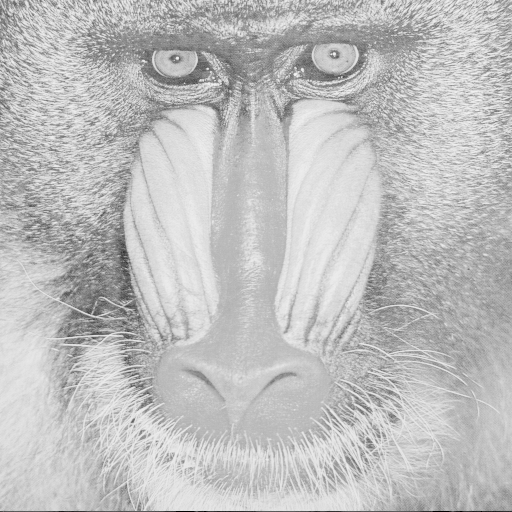
\includegraphics[width=6cm]{resultados/baboongama.png}
        \caption{\texttt{imagens/baboon.png}}
    \end{subfigure}

    \caption{Brilho ajustado com $\gamma = 2.5$.}
\end{figure}

\begin{listing}[H]
    \caption{Comando \texttt{aj.brilho GAMA}}

    \begin{minted}{python}
        def ajuste_brilho(imagem, gama):
            A = imagem / 255
            B = A ** (1 / gama)
            return (B * 255).astype(np.uint8)
    \end{minted}
\end{listing}

\subsection{Planos de Bit}

Extração de um plano de bit $M$ da imagem. O argumento $M$ deve aparecer logo após o comando, como em:

\begin{minted}{bash}
    $ python main.py imagens/baboon.png plano.bit 4
\end{minted}

\begin{listing}[H]
    \caption{Comando \texttt{plano.bit M}}

    \begin{minted}{python}
        def plano_de_bit(imagem, bit):
            plano = (imagem >> bit) & 1
            return plano * 255
    \end{minted}
\end{listing}

\begin{figure}[H]
    \centering
    \begin{subfigure}{0.45\textwidth}
        \centering
        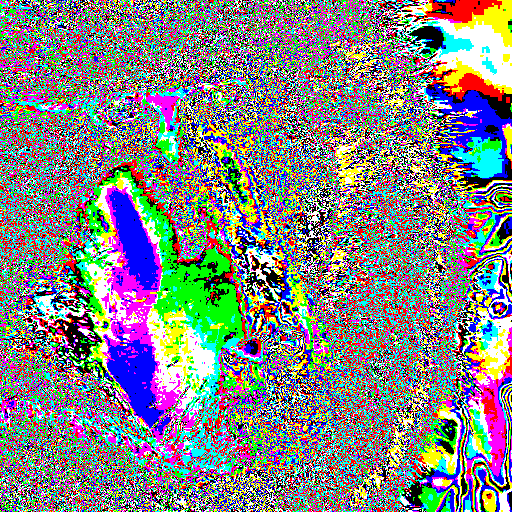
\includegraphics[width=6cm]{resultados/colorbit.png}
        \caption{\texttt{imagens/color.png}}
        \label{fig:ajbrilho}
    \end{subfigure}%
    \begin{subfigure}{0.45\textwidth}
        \centering
        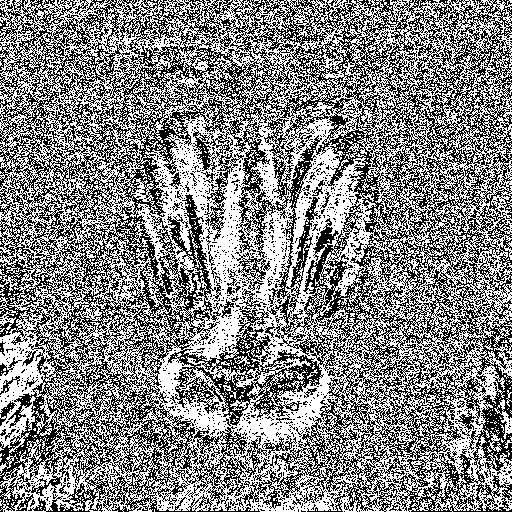
\includegraphics[width=6cm]{resultados/baboonbit.png}
        \caption{\texttt{imagens/babooon.png}}
    \end{subfigure}

    \caption{Plano de bit 4.}
\end{figure}

\subsection{Combinação de Imagens}

Combinação da imagem atual $A$ com uma segunda imagem $B$ com peso $\alpha$, resultando em $\alpha A + (1 - \alpha) B$. Tanto a imagem $B$ quanto o peso $\alpha$ devem ser passadao como argumentos, nessa ordem.

\begin{minted}{bash}
    $ python main.py imagens/baboon.png combina imagens/butterfly 0.2
\end{minted}

\begin{listing}[H]
    \caption{Comando \texttt{combina IMAGEM ALPHA}}

    \begin{minted}{python}
        def combinacao(A, B, alpha):
            img = A * alpha + B * (1 - alpha)
            return img.astype(np.uint8)
    \end{minted}
\end{listing}

\begin{figure}[H]
    \centering
    \begin{subfigure}{0.45\textwidth}
        \centering
        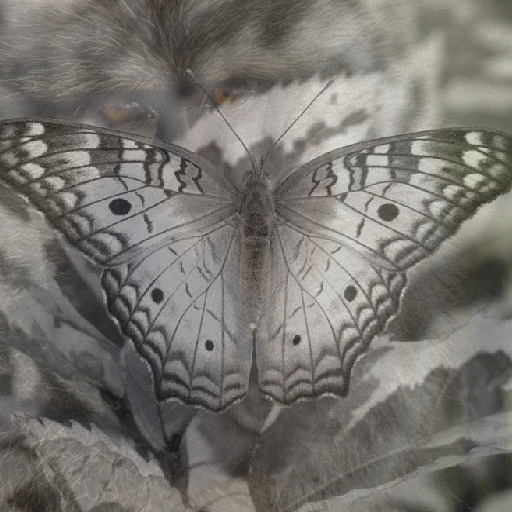
\includegraphics[width=6cm]{resultados/colormerg.png}
        \caption{\texttt{imagens/color.png}}
    \end{subfigure}%
    \begin{subfigure}{0.45\textwidth}
        \centering
        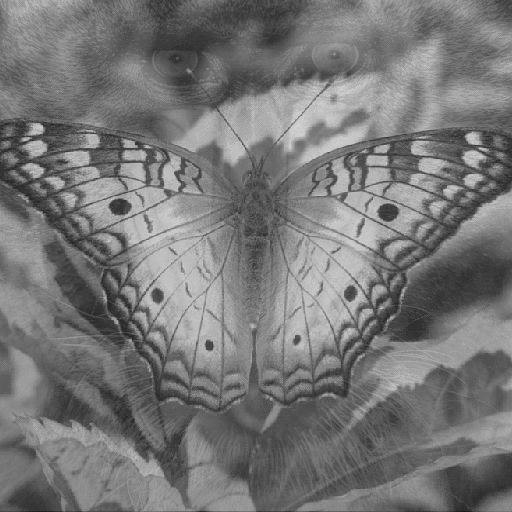
\includegraphics[width=6cm]{resultados/baboonmerg.png}
        \caption{\texttt{imagens/babooon.png}}
    \end{subfigure}

    \caption{Imagem combinada com \texttt{imagens/butterfly.png}, com $\alpha = 0.2$.}
\end{figure}

\subsection{Mosaico} \label{sec:mosaico}

\textcolor{red}{ORDENACAO? PADRAO? IMPL?}

\begin{minted}{text}
    $ python main.py imagens/baboon.png mosaico padrao.txt
\end{minted}

\begin{figure}[H]
    \centering
    \begin{subfigure}{0.45\textwidth}
        \centering
        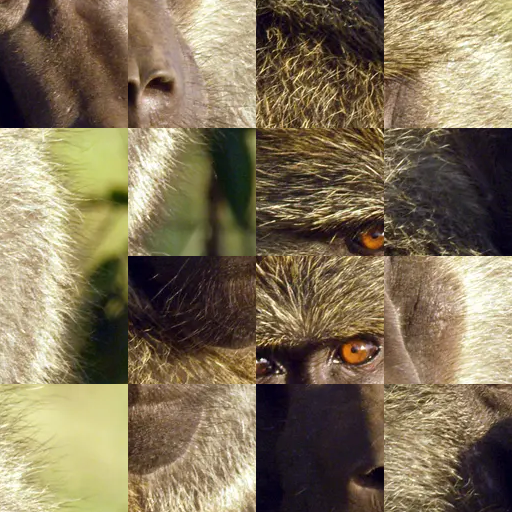
\includegraphics[width=6cm]{resultados/colormsc.png}
        \caption{\texttt{imagens/color.png}}
    \end{subfigure}%
    \begin{subfigure}{0.45\textwidth}
        \centering
        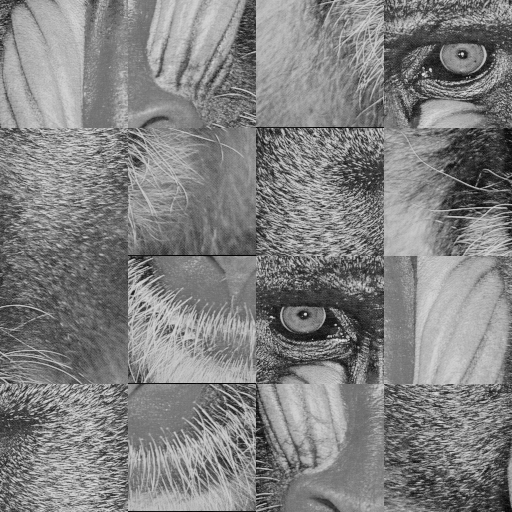
\includegraphics[width=6cm]{resultados/baboonmsc.png}
        \caption{\texttt{imagens/babooon.png}}
        \label{fig:res:10}
    \end{subfigure}

    \caption{Mosaico da imagem com \textcolor{red}{ALGUMA COISA}.}
\end{figure}

\begin{listing}[H]
    \begin{minted}{python}
        def mosaico(imagem, ordem):
            N, M = ordem.shape
            # split e flatten
            bloco = [
                bloco
                for lin in np.vsplit(imagem, N)
                for bloco in np.hsplit(lin, M)
            ]
            # accesso (em lista) e concatena
            imagem = np.concatenate([
                np.concatenate([bloco[i] for i in lin], axis=1)
                for lin in ordem
            ])
            return imagem
    \end{minted}

    \caption{Comando \texttt{mosaico ORDENACAO}}
\end{listing}

